\documentclass[12pt,a4paper,oneside]{abntex2}

% PACOTES

% Pacotes fundamentais
\usepackage{cmap}	% Mapear caracteres especiais no PDF
\usepackage{lmodern}	% Usa a fonte Latin Modern
\usepackage[T1]{fontenc}	% Selecao de codigos de fonte.
\usepackage[utf8]{inputenc}	% Codificacao do documento (conversão automática dos acentos)
\usepackage{lastpage}	% Usado pela Ficha catalográfica
\usepackage{indentfirst}	% Indenta o primeiro parágrafo de cada seção.
\usepackage{color}	% Controle das cores
\usepackage{graphicx}	% Inclusão de gráficos
\usepackage{amsmath}	% Pacote para equações multi linhas
\usepackage{listings} % Inserção de código fonte
\usepackage{pgfplots}
\pgfplotsset{width=7cm,compat=1.13}

% Configurações do pacote 'listings'
\lstset{
	showspaces = false, % Marcar espaços
	showstringspaces = false, % Marcar os espaços nas strings
	showtabs = false, % Marcar tabs
	numbers = left, % Posição dos números de linha (Remova para eles desaparecerem)
	tabsize = 2, % Número de espaços por tab
	mathescape = true % Permite o ambiente de equações
}
% --------------------------------
% Para mais configurações do listings visite a página da wiki em
% http://en.wikibooks.org/wiki/LaTeX/Source_Code_Listings
% ou a documentação mais detalhada do pacote em
% ftp://ftp.tex.ac.uk/tex-archive/macros/latex/contrib/listings/listings.pdf
% --------------------------------

% Pacotes adicionais
\usepackage{lipsum}	% para geração de dummy text

% Comandos adicionais
\providecommand{\imprimirdisciplina}{}
\newcommand{\disciplina}[1]{\renewcommand{\imprimirdisciplina}{#1}}

% Informações do aluno e documento
\titulo{Trabalho}
\autor{Aluno:}
\disciplina{Processamento Digital de Sinais}
\orientador{Kennedy Reurison Lopes}

% Configurações de aparência do PDF final
\definecolor{blue}{RGB}{41,5,195} % alterando o aspecto da cor azul

% informações do PDF
\makeatletter
\hypersetup{
     	%pagebackref=true,
		pdftitle={\@title},
		pdfauthor={\@author},
    	pdfsubject={\@title},
	    pdfcreator={LaTeX with abnTeX2},
		pdfkeywords={abnt}{latex}{abntex}{abntex2}{lista de exercícios},
		colorlinks=true,       		% false: boxed links; true: colored links
    	linkcolor=blue,          	% color of internal links
    	citecolor=blue,        		% color of links to bibliography
    	filecolor=magenta,      		% color of file links
		urlcolor=blue,
		bookmarksdepth=4
}
\makeatother

\setlength{\parindent}{0cm} % Remove indentação dos parágrafos
\setlength{\parskip}{0.5cm} % Espaçamento entre parágrafos

% Novo estilo de cabeçalho com a identificação do aluno
\makepagestyle{cabidaluno}
	% Cabeçalhos
	\makeoddhead{cabidaluno}
		{\imprimirautor}{\imprimirtitulo}{\thepage}
	\makeevenhead{cabidaluno}
		{\imprimirautor}{\imprimirtitulo}{\thepage}
	\makeheadrule{cabidaluno}{\textwidth}{\normalrulethickness} % linha separadora
	% Rodapé
	\makeoddfoot{cabidaluno}
		{\imprimirorientador\ -- \imprimirdisciplina\ -- \today}{}{}
	\makeevenfoot{cabidaluno}
		{\imprimirorientador\ -- \imprimirdisciplina\ -- \today}{}{}
% INICIO DO DOCUMENTO

\begin{document}

	% Elementos textuais
	\textual
	\pagestyle{cabidaluno} % Inclusão de cabeçalhos e rodapés personalizados
	
1) Determine qual será a região de convergência, caso exista, necessária para que:


\pgfplotsset{compat=1.13}
\begin{center}
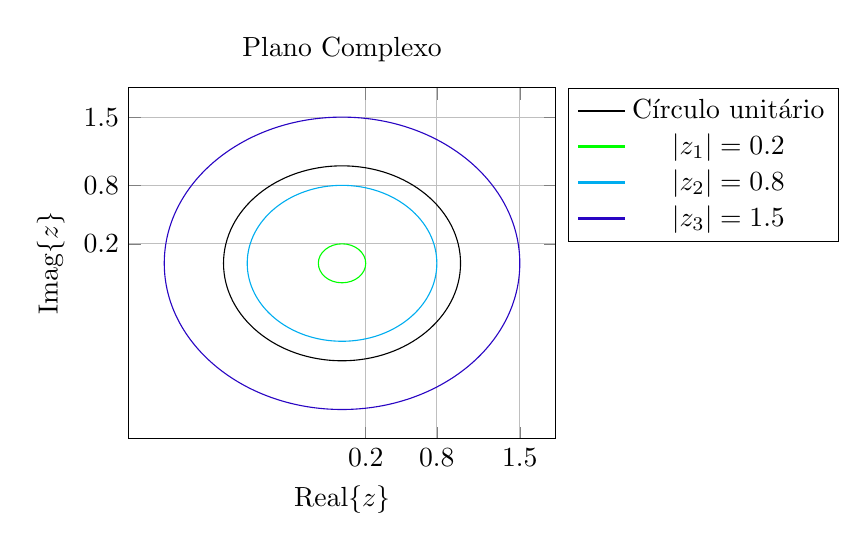
\begin{tikzpicture}
 \begin{axis}[enlargelimits,
  xmin=-1.5,xmax=1.5,
  ymin=-1.5,ymax=1.5,
  xtick={0.2,0.8,1.5},
  ytick={0.2,0.8,1.5},
  grid=major,
  title=Plano Complexo,
  xlabel=Real$\{z\}$,
  ylabel=Imag$\{z\}$,
  legend pos=outer north east,
]
  \draw[black] (0,0) circle[radius=1];
  \draw[cyan] (0,0) circle[radius=0.8];
  \draw[green] (0,0) circle[radius=0.2];
  \draw[blue] (0,0) circle[radius=1.5];
  \addlegendimage{line width=0.3mm,color=black}
  \addlegendentry{Círculo unitário}
  \addlegendimage{line width=0.3mm,color=green}
  \addlegendentry{$|z_1| = 0.2$}
  \addlegendimage{line width=0.3mm,color=cyan}
  \addlegendentry{$|z_2| = 0.8$}
  \addlegendimage{line width=0.3mm,color=blue}
  \addlegendentry{$|z_3| = 1.5$}
\end{axis}
\end{tikzpicture}
\end{center}

a) O sistema seja Causal e estável.\\
b) O sistema seja Causal e instável.\\
c) O sistema seja não Causal e estável.\\
d) O sistema seja não Causal e instável


\end{document}